ANTS supports both volumetric registration and point set registration. The image / point set similarity metrics in ANTS are unified in the form of a function on the images or the point sets:       $$\textbf{Simlarity}[\textbf{fixedImage}, \textbf{movingImage}, \textbf{weight}, \textbf{parameters}].$$
        
The similarity type for the deformation transformation is specified by \verb -m  option, which contains two parts: simarity type and the parameters inside the brackets. (Note: no white spaces exist between parameters.) The possible similarity metrics for volumetric images are: 
\begin{itemize}
    \item Cross correlation estimate:  \verb"-m CC[fixedImage,movingImage,weight,radius]". This metric works well for intra-modality image registration. For exxample, \verb"-m CC[fixed.nii,moving.nii,1,5]" specifies:
    \begin{itemize}
        \item the fixed image: fixed.nii
        \item the moving image: moving.nii             
        \item weight for this metric is 1 (i.e. only this metric drives the registration).      
        \item the region radius for computing cross correlation is 5
    \end{itemize}

    \item Mutual information: \verb"-m MI[fixedImage,movingImage,weight,number-of-histogram-bins]". This metric works both well for intra-modality and inter-modality image registration. For example, the first three parameters in \verb"-m MI[fixed.nii,moving.nii,1,32]" is similar to the example above in cross correlation, except that the last parameter means that the number of bins in computing mutual information is 32.

    \item PR: \verb"-m PR[fixedImage,movingImage,weight,radius]". This metric works for intra-modality image registration and some inter-modality cases. This metric is a strict implementation of correlation whereas CC estimates correlation-like optical flow. The meaning of parameters are similar to cross correlation.

    \item Mean square difference: \verb"-m MSQ[fixedImage,movingImage,weight,0]". This metric works for intra-modality image registration. The last parameter \verb"0" is a padding value of no real meaning. For example, \verb"-m MSQ[fixed.nii,moving.nii,1,0]". 

\end{itemize}

ANTS also support registration of point sets. The supported formats for point sets can be found in I/O section. The similarity metrics for point sets are:
\begin{itemize}
    \item Point set expectation: 
     \begin{verbatim}
-m PSE [fixedImage,movingImage,fixedPoints,movingPoints,weight,
pointSetPercentage,pointSetSigma,boundaryPointsOnly,
kNeighborhood,PartialMatchingIterations=100000]
    \end{verbatim}
    \begin{itemize}
        \item \verb"fixedImage": defines the space domain of the fixed point set.
        \item \verb"movingImage": defines the space domain of the moving point set.
        \item \verb"fixedPoints/Image": defines the coordinates of the fixed point set or label image. It can be an image with discrete positive labels, a VTK format point set file, or a text file. Details can be found in I/O section (TODO).
        \item \verb"movingPoints/Image": defines the coordinates of the moving point set or label image. 
        \item \verb"weight": weight for this metric. \verb"1" means that only this metric drives the registration.
        \item \verb"pointSetPercentage": the percentage of points to be randomly sampled used in the registration.
        \item \verb"pointSetSigma": the standard deviation of the Parzen window used to estimate the expectation. 
        \item \verb"boundaryPointsOnly":  \verb"1" (or ``true'') means only the boundary points in the label image is used to drive registration.
        \item \verb"kNeighborhood" is a positive discrete number. The first $k$ neighbors are used to compute the deformation during the registration. 
        \item \verb"PartialMatchingIterations" controls the symmtry in the matching. This option assumes the complete labeling is in the first set of label parameters ... more iterations leads to more symmetry in the matching  - 0 iterations means full asymmetry 
    \end{itemize}

    \item Jensen-Tsallis BSpline
    \begin{verbatim}
-m JTB[fixedImage,movingImage,fixedPoints,movingPoints,weight,
pointSetPercentage,pointSetSigma,boundaryPointsOnly,kNeighborhood,alpha,
meshResolution,splineOrder,numberOfLevels,useAnisotropicCovariances] 
    \end{verbatim}
    \begin{itemize}
        \item \verb"fixedImage": defines the space domain of the fixed point set.
        \item \verb"movingImage": defines the space domain of the moving point set.
        \item \verb"fixedPoints": defines the coordinates of the fixed point set. It can be an image with discrete positive labels, a VTK format point set file, or a text file. Details can be found in I/O section (TODO).
        \item \verb"movingPoints": defines the coordinates of the moving point set.
        \item \verb"weight": weight for this metric. \verb"1" means that only this metric drives the registration.
        \item \verb"pointSetPercentage": the percentage of points to be randomly sampled used in the registration.
        \item \verb"pointSetSigma": the sigma for the Parzen window used to estimate probabilities.  
        \item \verb"boundaryPointsOnly": [TODO] \verb"1" (or ``true'') means only the boundary points in the point sets are used to drive registration.
        \item \verb"kNeighborhood" is a positive discrete number. The first $k$ neighbors are used to compute the deformation during the registration. 
        \item \verb"alpha"
        \item \verb"meshResolution"
        \item \verb"splineOrder"
        \item \verb"numberOfLevels"
        \item \verb"useAnisotropicCovariances"
    \end{itemize}

\end{itemize}

In current implementation, the affine registration only supports two types of similarity metrics on volumetric images, which are specified using \verb"--affine-metric-type":
\begin{itemize}
    \item Mutual information, specified as \verb"--affine-metric-type MI". This usually works for both inter and intra-modalities in 3D. Also, the options used in computing mututal information in affine registration can be specified as \verb"--MI-option N1xN2". The first parameter \verb"N1" specifies the number of bins. The second parameter \verb"N2" specifies the number of samples. For example: \verb"--MI-option 32x8000".

    \item Mean square difference, specified using \verb"--affine-metric-type MSE". There is no options for this metric.
\end{itemize}

Fig. \ref{fig:metric_example} shows the registration result using intensity difference with the following command:
\begin{verbatim}
ANTS 2 -m MSQ[r16slice.nii,r64slice.nii,1,0] -r Gauss[3,0] -t SyN[0.5] -i 50x50x30
\end{verbatim}

%        \begin{wrapfigure}{r}{0.5\textwidth}
\begin{figure}
    \label{fig:metric_example}
    \centering
    \begin{tabular}[h]{c|c|c}
%        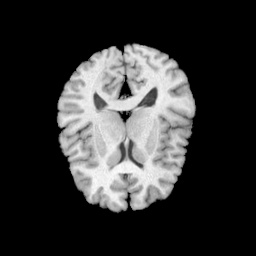
\includegraphics[width=0.16\textwidth]{Figures/r16slice.jpg} &
%        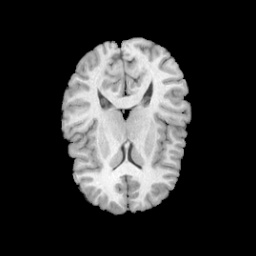
\includegraphics[width=0.16\textwidth]{Figures/r64slice.jpg} &
 %       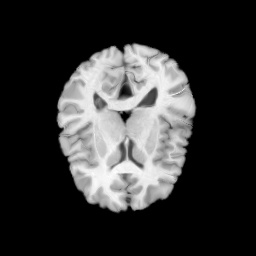
\includegraphics[width=0.16\textwidth]{Figures/resMSQ.jpg} \\
        fixed image &
        moving image & 
        MSE  \\
    \end{tabular} 
    \itkcaption{registration using mean square intensity difference}
\end{figure}
    %    \end{wrapfigure}
Here is also an example script to register a pair of images using mean square intensity difference and computing the metrics of the registration image.
\begin{verbatim}
#use intensity difference with radius 0 -- radius no effect on intensity difference
ANTS 2 -m MSQ[r16slice.nii,r64slice.nii,1,0] -r Gauss[3,0] -t SyN[0.5] -i 50x50x30
WarpImageMultiTransform 2 r64slice.nii resMSQ.nii Warp.nii Affine.txt
MeasureImageSimilarity 2 0 r16slice.nii resMSQ.nii metricexamplelog.txt
MeasureImageSimilarity 2 1 r16slice.nii resMSQ.nii metricexamplelog.txt
MeasureImageSimilarity 2 2 r16slice.nii resMSQ.nii metricexamplelog.txt
ConvertToJpg resMSQ.nii resMSQ.jpg
\end{verbatim}
